\renewcommand{\thefootnote}{\fnsymbol{footnote}}

\chapter[Introduction to uncertainty]%
 {Introduction to uncertainty}
\label{ch:L1}

% 3) Reset things so later footnotes go back to 1, 2, 3, …
\setcounter{footnote}{0}
\renewcommand{\thefootnote}{\arabic{footnote}}

\section{How to model uncertainty}\label{sec:L1-intro}

The outcomes of our decisions are often uncertain, so we want a choice theory that takes uncertainty into account. Let's start by thinking about how to represent uncertainty. Suppose you make a bet with a friend: if a fair coin toss results in heads, you get \(10\) euros; otherwise you pay \(10\) euros to your friend. There are two outcomes, \(10\) and \(-10\), and since the coin is fair, each occurs with probability \(\nicefrac{1}{2}\). What are the main ingredients of this example?

First, we started from a set of outcomes, in this case the monetary transfers \(10\) and \(-10\). Second, we specified the probability of each outcome occurring, \(\nicefrac{1}{2}\) for both. We call such an object—a set of outcomes, each associated with a probability—a \textbf{lottery}. Denote the set of outcomes by \(X\). Generic elements of \(X\) will be denoted \(x,y,z\) or sometimes \(x_1, x_2, \dots\). For simplicity, assume that \(X\) is finite. Outcomes alone are not enough to describe a lottery: we need probability distributions over outcomes, as in the \(\nicefrac{1}{2}\)–\(\nicefrac{1}{2}\) distribution of the fair coin above. The set of lotteries over \(X\) is denoted by \(\Delta(X)\).\footnote{Why the notation \(\Delta\)? You will realise soon.} Each element of \(\Delta(X)\) is a function \(p:X\to[0,1]\) such that \(\sum_{x\in X} p(x)=1\); it maps each outcome \(x\) to a number \(p(x)\in[0,1]\), representing the probability that \(x\) occurs.\footnote{Why do we write a sum \(\sum_{x\in X} p(x)=1\) and not an integral?} We can write a lottery as a vector, for example \(p=(p(x),p(y),p(z))\) if \(X=\{x,y,z\}\).

\begin{example}\label{ex:coin}
	In the example above, the set of outcomes is \(\{10,-10\}\) and the lottery \(p\in\Delta(\{10,-10\})\) induced by the fair coin toss satisfies \(p(10)=p(-10)=\nicefrac{1}{2}\).
\end{example}

We can depict lotteries using a tree diagram, as in Figure~\ref{fig:lottery-tree}.

\tikzset{every picture/.style={line width=0.75pt}} % default line width        
\begin{figure}[H]
	\centering
	\begin{tikzpicture}[>=stealth, x=1cm, y=1cm]
		% coordinates
		\coordinate (root) at (0,0);
		\coordinate (up)   at (3,1.2);
		\coordinate (down) at (3,-1.2);

		% branches
		\draw (root) -- (up)   node[midway, above] {$\tfrac{1}{2}$} node[right] {$10$};
		\draw (root) -- (down) node[midway, below] {$\tfrac{1}{2}$} node[right] {$-10$};

		% root dot
		\fill (root) circle (1.5pt);
	\end{tikzpicture}
	\caption{Lottery from Example \ref{ex:coin}.}
	\label{fig:lottery-tree}
\end{figure}

\begin{remark}
	Notice that, in this setup, we are missing something: whether the coin lands on heads or tails is irrelevant; only the probabilities of outcomes matter, not the events that induced them. This is a limitation of this model, which we will address when we introduce a state-space representation of uncertainty.
\end{remark}

The set of lotteries \(\Delta(X)\) has \emph{structure}: we can combine its elements in a meaningful way. For example, consider a lottery \(r\) that yields the lottery \(p\) with probability \(\alpha\) and \(q\) with probability \(1-\alpha\), where \(\alpha\in[0,1]\). This is a \textit{compound lottery}. It is still an element of \(\Delta(X)\), and we write \(r=\alpha p+(1-\alpha)q\). For instance, if \(p(10)=\nicefrac{1}{2}\) and \(q(10)=\nicefrac{1}{4}\), the associated compound lottery is represented on the left of Figure~\ref{fig:compound-lottery-tree}. We can compute the probability that outcome \(10\) occurs in this compound lottery: \(\alpha\times\nicefrac{1}{2}+(1-\alpha)\times\nicefrac{1}{4}=\tfrac{1+\alpha}{4}\). By computing the probability of each outcome in a compound lottery, we \emph{reduce} it to a simple lottery, as represented on the right of Figure~\ref{fig:compound-lottery-tree}.

\begin{figure}[H]
	\centering
	\begin{tikzpicture}[>=stealth, x=1cm, y=1cm]
		% styles
		\tikzset{
			dot/.style={circle, fill, inner sep=1.2pt},
			lottery/.style={circle, draw, inner sep=1.6pt},
		}

		%=== left: compound lottery ===%
		% coordinates
		\coordinate (root)  at (0,0);
		\coordinate (p)     at (3, 1.5);
		\coordinate (q)     at (3,-1.5);

		\coordinate (p10)   at (6, 2.5);
		\coordinate (p-10)  at (6, 0.5);
		\coordinate (q10)   at (6,-0.5);
		\coordinate (q-10)  at (6,-2.5);

		% nodes
		\node[dot] at (root) {};
		\node[lottery, label=above:$p$]  (pnode) at (p) {};
		\node[lottery, label=below:$q$]  (qnode) at (q) {};

		% stage 1
		\draw (root) -- (pnode) node[midway, above] {$\alpha$};
		\draw (root) -- (qnode) node[midway, below] {$1-\alpha$};

		% stage 2 from p
		\draw (pnode) -- (p10)  node[midway, above] {$\tfrac{1}{2}$} node[right] {$10$};
		\draw (pnode) -- (p-10) node[midway, below] {$\tfrac{1}{2}$} node[right] {$-10$};

		% stage 2 from q
		\draw (qnode) -- (q10)  node[midway, above] {$\tfrac{1}{4}$} node[right] {$10$};
		\draw (qnode) -- (q-10) node[midway, below] {$\tfrac{3}{4}$} node[right] {$-10$};

		%=== right: reduced (simple) lottery r ===%
		\coordinate (rroot) at (9.6,0);
		\coordinate (r10)   at (12.6, 1.5);
		\coordinate (r-10)  at (12.6,-1.5);

		\node[dot] at (rroot) {};
		\node[above=2pt] at (rroot) {$r$};

		\draw (rroot) -- (r10)
		node[midway, above] {$\displaystyle \frac{1+\alpha}{4}$}
		node[right] {$10$};

		\draw (rroot) -- (r-10)
		node[midway, below] {$\displaystyle \frac{3-\alpha}{4}$}
		node[right] {$-10$};
	\end{tikzpicture}

	\caption{Compound lottery (left) and its reduced form (right).}
	\label{fig:compound-lottery-tree}
\end{figure}

We assume \emph{reduction of compound lotteries}: individuals are indifferent between any compound lottery and its reduced form, i.e., any two lotteries that induce the same probabilities over outcomes are treated as the same.

\begin{techremark}
	Can you think of reasons why someone might \emph{not} be indifferent between a compound lottery and its reduced form? Violations of reduction generate interesting phenomena studied in behavioural economics. See, e.g., \citet{segalTwostageLotteriesReduction1990} and \citet{dillenbergerAdditivebeliefbasedPreferences2020}.
\end{techremark}

This lottery \emph{mixing} operation is not possible with an unstructured set of outcomes. As an illustration, suppose the set of outcomes comprises fruits. We can have an apple or a banana, but there is no fruit that is a mixture of an apple and a banana. Imposing structure on the set of elements to be ranked is a key move of microeconomic theory. In fact, we will later assume that the set of outcomes is \(\mathbb{R}\), the set of real numbers representing monetary outcomes, which lets us say more than with a generic set of outcomes.

There is another way to represent lotteries graphically. Consider once again the coin toss: obtaining \(10\) euros with probability \(\nicefrac{1}{2}\) and \(-10\) euros with probability \(\nicefrac{1}{2}\). We can represent this lottery as the midpoint of the line segment whose endpoints correspond to the degenerate lotteries yielding \(10\) and \(-10\) with probability \(1\); see panel~(a) of Figure~\ref{fig:lottery-simplex-stacked}. More generally, with \(n\) outcomes we can represent a lottery as a point in an \((n-1)\)-dimensional simplex. For example, with three outcomes we can represent lotteries as points in an equilateral triangle, as in panel~(b).\footnote{That's why the \( \Delta \) notation!} The vertices of the triangle correspond to degenerate lotteries that yield one outcome with probability \(1\). Any other point in the triangle corresponds to a lottery that yields each of the three outcomes with some probability. Roughly, the farther a point is from a vertex, the lower the probability of the corresponding outcome. For example, the lottery \(p\) in panel~(b) yields outcome \(x\) with relatively high probability and outcomes \(y\) and \(z\) with relatively low probabilities.

\begin{figure}[H]
	\centering
	\begin{tikzpicture}[x=1cm,y=1cm,>=stealth]
		\tikzset{dot/.style={circle,fill,inner sep=1.5pt}}

		\begin{scope}
			\coordinate (L) at (0,0);
			\coordinate (R) at (6,0);
			\draw[thick] (L)--(R);

			% endpoints
			\node[dot] at (L) {};
			\node[dot] at (R) {};
			\node[below=6pt] at (L) {$10$};
			\node[below=6pt] at (R) {$-10$};

			% midpoint and label
			\coordinate (M) at ($(L)!0.5!(R)$);
			\node[dot] at (M) {};
			\node[above=6pt] at (M) {$p(10)=p(-10)=\tfrac{1}{2}$};

			% centered panel caption
			\node at ($(L)!0.5!(R)+(0,-1.1)$) {\small (a) Two outcomes};
		\end{scope}


		%---------------- BOTTOM: three-outcome lottery in a triangle -------%
		\begin{scope}[yshift=-8.8cm]
			\coordinate (A) at (0,0);
			\coordinate (B) at (6,0);
			\coordinate (C) at (3,5.196); % sqrt(3)/2 * 6
			\draw[thick] (A)--(B)--(C)--cycle;

			% vertex labels = degenerate lotteries
			\node[dot] at (A) {};
			\node[below,align=center] at (A) {$x$ \\ {\scriptsize $(1,0,0)$}};
			\node[dot] at (B) {};
			\node[below,align=center] at (B) {$y$ \\ {\scriptsize $(0,1,0)$}};
			\node[dot] at (C) {};
			% put the coordinate first, then z, so z is closer to the vertex
			\node[above,align=center] at (C) {{\scriptsize $(0,0,1)$}\\[-2pt] $z$};

			% a generic interior lottery
			\coordinate (P) at (1.5,0.8);
			\node[dot] at (P) {};
			\draw[->] ($(P)+(-0.55,0.35)$) -- (P);
			\node[right=3pt] at (P) {$\big(p(x),\,p(y),\,p(z)\big)$};

			\node at (3,-1.1) {\small (b) Three outcomes};
		\end{scope}

	\end{tikzpicture}
	\caption{Lotteries as points in simplexes: (a) a two–outcome lottery lies on a line segment; (b) with three outcomes, lotteries lie in an equilateral triangle.}
	\label{fig:lottery-simplex-stacked}
\end{figure}

\begin{techremark}
	For a finite outcome set \( X \), the probability simplex over \( X \) is

	\[
		\Delta(X)=\left\{p: X \rightarrow[0,1] \mid \sum_{x \in X} p(x)=1\right\}
	\]

	or equivalently

	\[
		\left\{\left(p\left(x_1\right), \ldots, p\left(x_n\right)\right) \in \mathbb{R}^n \mid p\left(x_i\right) \geq 0, \sum_i p\left(x_i\right)=1\right\}.
	\]

	This is an \(n-1 \)-dimensional simplex whose vertices are the degenerate lotteries (unit vectors), e.g. \( (1,0, \ldots, 0), \ldots,(0, \ldots, 0,1) \).
\end{techremark}

\section{Preferences over lotteries}

Our aim is to understand how individuals choose between lotteries, whether they like or dislike risk, and how to compare different individuals' attitudes towards risk. We therefore need to make statements such as \enquote{an individual weakly prefers lottery \(p\) to lottery \(q\)}. To do so, introduce a binary relation \(\succsim\) over \(\Delta(X)\), so that \(p\succsim q\) reads \enquote{the individual weakly prefers lottery \(p\) to lottery \(q\)}.\footnote{Are you curious why we use the symbol \( \succsim \) for preferences and not \( \geq \)? An historian of economic theory, \href{https://ivanboldyrev.net/}{Ivan Boldyrev}, told me it is from \cite{hersteinAxiomaticApproachMeasurable1953}, who used the symbol in their famous paper where they provided an axiomatic characterisation of expected utility, which we will do soon.} Compared to choice under certainty, we are now comparing lotteries—i.e., probability distributions over outcomes—rather than outcomes themselves.

\begin{techremark}
	Technically, \(\succsim\) is a subset of \(\Delta(X) \times \Delta(X)\), i.e., a set of ordered pairs of lotteries. For example, if \(p,q,r\in\Delta(X)\), the statements \emph{\(p\) is (weakly) preferred to \(q\)} imply \((p,q)\in\succsim\).
\end{techremark}

Recall that we can define strict preference and indifference in terms of weak preference: \(p\succ q\), which reads \textquote{\(p\) is strictly preferred to \(q\)} if and only if \(p\succsim q\) but not \(q\succsim p\); and \(p\sim q\), which reads \textquote{\(p\) is indifferent to \(q\)} if and only if both \(p\succsim q\) and \(q\succsim p\).

In what follows, we consider what assumptions preferences over lotteries might satisfy, and what these assumptions imply for behaviour.

\section{Things to read}

See \citet[pp.~31–33]{krepsNotesTheoryChoice1988} for a brief intuitive introduction to the lottery model in this chapter. If you want to read a similar treatment from a textbook read \citet[pp.~168–170]{mas-colellMicroeconomicTheory1995}.

\section{Exercises}

\begin{exercise}
	Can we still represent the set of lotteries and compound lotteries on the simplex if there is no indifference between a compound lottery and its reduced form? Why or why not?
\end{exercise}

\begin{exercise}
	Assume there are three outcomes \(x,y,z\). Draw in the simplex the set of lotteries that yield each outcome with the same probability and the lottery that yields \(x\) with certainty. Now draw the set of all mixtures of these two lotteries. Assume that the individual is indifferent between the lottery yielding each outcome with the same probability, the lottery yielding \(x\) with certainty, and any mixture of the two. Which part of the simplex does this indifference \textquote{curve} correspond to? Is it really a curve?
\end{exercise}

\begin{exercise}
	Assuming three outcomes \(x,y,z\), draw in the simplex the set of lotteries that yield outcome \(x\) with probability at least \(\nicefrac{1}{2}\).
\end{exercise}

\begin{exercise}
	In the main text we assumed that individuals are indifferent between a compound lottery and its reduced form. State this indifference formally as a condition on the preference relation \(\succsim\), using the notation introduced.
\end{exercise}

\bibliographystyle{apacite}  % or another  style
\bibliography{references} % .bib file goes in ./bib/